% Options for packages loaded elsewhere
\PassOptionsToPackage{unicode}{hyperref}
\PassOptionsToPackage{hyphens}{url}
%
\documentclass[
]{article}
\title{Science Curiosity Study 1 Data}
\author{}
\date{\vspace{-2.5em}}

\usepackage{amsmath,amssymb}
\usepackage{lmodern}
\usepackage{iftex}
\ifPDFTeX
  \usepackage[T1]{fontenc}
  \usepackage[utf8]{inputenc}
  \usepackage{textcomp} % provide euro and other symbols
\else % if luatex or xetex
  \usepackage{unicode-math}
  \defaultfontfeatures{Scale=MatchLowercase}
  \defaultfontfeatures[\rmfamily]{Ligatures=TeX,Scale=1}
\fi
% Use upquote if available, for straight quotes in verbatim environments
\IfFileExists{upquote.sty}{\usepackage{upquote}}{}
\IfFileExists{microtype.sty}{% use microtype if available
  \usepackage[]{microtype}
  \UseMicrotypeSet[protrusion]{basicmath} % disable protrusion for tt fonts
}{}
\makeatletter
\@ifundefined{KOMAClassName}{% if non-KOMA class
  \IfFileExists{parskip.sty}{%
    \usepackage{parskip}
  }{% else
    \setlength{\parindent}{0pt}
    \setlength{\parskip}{6pt plus 2pt minus 1pt}}
}{% if KOMA class
  \KOMAoptions{parskip=half}}
\makeatother
\usepackage{xcolor}
\IfFileExists{xurl.sty}{\usepackage{xurl}}{} % add URL line breaks if available
\IfFileExists{bookmark.sty}{\usepackage{bookmark}}{\usepackage{hyperref}}
\hypersetup{
  pdftitle={Science Curiosity Study 1 Data},
  hidelinks,
  pdfcreator={LaTeX via pandoc}}
\urlstyle{same} % disable monospaced font for URLs
\usepackage[margin=1in]{geometry}
\usepackage{color}
\usepackage{fancyvrb}
\newcommand{\VerbBar}{|}
\newcommand{\VERB}{\Verb[commandchars=\\\{\}]}
\DefineVerbatimEnvironment{Highlighting}{Verbatim}{commandchars=\\\{\}}
% Add ',fontsize=\small' for more characters per line
\usepackage{framed}
\definecolor{shadecolor}{RGB}{248,248,248}
\newenvironment{Shaded}{\begin{snugshade}}{\end{snugshade}}
\newcommand{\AlertTok}[1]{\textcolor[rgb]{0.94,0.16,0.16}{#1}}
\newcommand{\AnnotationTok}[1]{\textcolor[rgb]{0.56,0.35,0.01}{\textbf{\textit{#1}}}}
\newcommand{\AttributeTok}[1]{\textcolor[rgb]{0.77,0.63,0.00}{#1}}
\newcommand{\BaseNTok}[1]{\textcolor[rgb]{0.00,0.00,0.81}{#1}}
\newcommand{\BuiltInTok}[1]{#1}
\newcommand{\CharTok}[1]{\textcolor[rgb]{0.31,0.60,0.02}{#1}}
\newcommand{\CommentTok}[1]{\textcolor[rgb]{0.56,0.35,0.01}{\textit{#1}}}
\newcommand{\CommentVarTok}[1]{\textcolor[rgb]{0.56,0.35,0.01}{\textbf{\textit{#1}}}}
\newcommand{\ConstantTok}[1]{\textcolor[rgb]{0.00,0.00,0.00}{#1}}
\newcommand{\ControlFlowTok}[1]{\textcolor[rgb]{0.13,0.29,0.53}{\textbf{#1}}}
\newcommand{\DataTypeTok}[1]{\textcolor[rgb]{0.13,0.29,0.53}{#1}}
\newcommand{\DecValTok}[1]{\textcolor[rgb]{0.00,0.00,0.81}{#1}}
\newcommand{\DocumentationTok}[1]{\textcolor[rgb]{0.56,0.35,0.01}{\textbf{\textit{#1}}}}
\newcommand{\ErrorTok}[1]{\textcolor[rgb]{0.64,0.00,0.00}{\textbf{#1}}}
\newcommand{\ExtensionTok}[1]{#1}
\newcommand{\FloatTok}[1]{\textcolor[rgb]{0.00,0.00,0.81}{#1}}
\newcommand{\FunctionTok}[1]{\textcolor[rgb]{0.00,0.00,0.00}{#1}}
\newcommand{\ImportTok}[1]{#1}
\newcommand{\InformationTok}[1]{\textcolor[rgb]{0.56,0.35,0.01}{\textbf{\textit{#1}}}}
\newcommand{\KeywordTok}[1]{\textcolor[rgb]{0.13,0.29,0.53}{\textbf{#1}}}
\newcommand{\NormalTok}[1]{#1}
\newcommand{\OperatorTok}[1]{\textcolor[rgb]{0.81,0.36,0.00}{\textbf{#1}}}
\newcommand{\OtherTok}[1]{\textcolor[rgb]{0.56,0.35,0.01}{#1}}
\newcommand{\PreprocessorTok}[1]{\textcolor[rgb]{0.56,0.35,0.01}{\textit{#1}}}
\newcommand{\RegionMarkerTok}[1]{#1}
\newcommand{\SpecialCharTok}[1]{\textcolor[rgb]{0.00,0.00,0.00}{#1}}
\newcommand{\SpecialStringTok}[1]{\textcolor[rgb]{0.31,0.60,0.02}{#1}}
\newcommand{\StringTok}[1]{\textcolor[rgb]{0.31,0.60,0.02}{#1}}
\newcommand{\VariableTok}[1]{\textcolor[rgb]{0.00,0.00,0.00}{#1}}
\newcommand{\VerbatimStringTok}[1]{\textcolor[rgb]{0.31,0.60,0.02}{#1}}
\newcommand{\WarningTok}[1]{\textcolor[rgb]{0.56,0.35,0.01}{\textbf{\textit{#1}}}}
\usepackage{graphicx}
\makeatletter
\def\maxwidth{\ifdim\Gin@nat@width>\linewidth\linewidth\else\Gin@nat@width\fi}
\def\maxheight{\ifdim\Gin@nat@height>\textheight\textheight\else\Gin@nat@height\fi}
\makeatother
% Scale images if necessary, so that they will not overflow the page
% margins by default, and it is still possible to overwrite the defaults
% using explicit options in \includegraphics[width, height, ...]{}
\setkeys{Gin}{width=\maxwidth,height=\maxheight,keepaspectratio}
% Set default figure placement to htbp
\makeatletter
\def\fps@figure{htbp}
\makeatother
\setlength{\emergencystretch}{3em} % prevent overfull lines
\providecommand{\tightlist}{%
  \setlength{\itemsep}{0pt}\setlength{\parskip}{0pt}}
\setcounter{secnumdepth}{-\maxdimen} % remove section numbering
\usepackage{booktabs}
\usepackage{longtable}
\usepackage{array}
\usepackage{multirow}
\usepackage{wrapfig}
\usepackage{float}
\usepackage{colortbl}
\usepackage{pdflscape}
\usepackage{tabu}
\usepackage{threeparttable}
\usepackage{threeparttablex}
\usepackage[normalem]{ulem}
\usepackage{makecell}
\usepackage{xcolor}
\ifLuaTeX
  \usepackage{selnolig}  % disable illegal ligatures
\fi

\begin{document}
\maketitle

\hypertarget{demographics}{%
\section{Demographics}\label{demographics}}

N\(_{total}\) = 541: N\(_{con}\) = 226, N\(_{lib}\) = 265, N\(_{mod}\) =
50

\textbf{N\(_{final}\) = 491}

\begin{itemize}
\tightlist
\item
  \textbf{Political ideology:} 46.03\% conservative, 53.97\% liberal
\item
  \textbf{Age:} Mean\(_{age}\) = 43.23 (range: 21-78)
\item
  \textbf{Gender:} 41.77\% women, 47.87\% men, 0.37\% non-binary folks,
  0.74\% preferred not to answer
\item
  \textbf{Race:} 75.05\% White, 5.36\% Black, 2.59\% Hispanic, 5.91\%
  Asian
\end{itemize}

\hypertarget{descriptives}{%
\section{Descriptives}\label{descriptives}}

\hypertarget{summary}{%
\subsection{Summary}\label{summary}}

\begin{tabular}{>{}l||>{}c|c|>{}c|c|>{}c}
\hline
  & Mean & SE & Min & Max & Median\\
\hline
\textbf{SciCuriosity} & \cellcolor{lightgray}{24.73} & 0.26 & \cellcolor{lightgray}{9} & 44 & \cellcolor{lightgray}{25}\\
\hline
\textbf{RPM} & \cellcolor{lightgray}{5.64} & 0.07 & \cellcolor{lightgray}{1} & 10 & \cellcolor{lightgray}{6}\\
\hline
\textbf{ConArctic} & \cellcolor{lightgray}{-1.43} & 0.06 & \cellcolor{lightgray}{-3} & 3 & \cellcolor{lightgray}{-2}\\
\hline
\textbf{ConTemp} & \cellcolor{lightgray}{-1.69} & 0.05 & \cellcolor{lightgray}{-3} & 3 & \cellcolor{lightgray}{-2}\\
\hline
\textbf{LibOzone} & \cellcolor{lightgray}{-0.26} & 0.06 & \cellcolor{lightgray}{-3} & 3 & \cellcolor{lightgray}{-1}\\
\hline
\textbf{LibAir} & \cellcolor{lightgray}{-0.82} & 0.07 & \cellcolor{lightgray}{-3} & 3 & \cellcolor{lightgray}{-1}\\
\hline
\textbf{ConFillIce} & \cellcolor{lightgray}{-2.10} & 0.05 & \cellcolor{lightgray}{-3} & 3 & \cellcolor{lightgray}{-2}\\
\hline
\textbf{FillBacteria} & \cellcolor{lightgray}{-0.27} & 0.06 & \cellcolor{lightgray}{-3} & 3 & \cellcolor{lightgray}{0}\\
\hline
\textbf{FillQuake} & \cellcolor{lightgray}{0.31} & 0.02 & \cellcolor{lightgray}{0} & 1 & \cellcolor{lightgray}{0}\\
\hline
\end{tabular}

\hypertarget{correlations}{%
\subsection{Correlations}\label{correlations}}

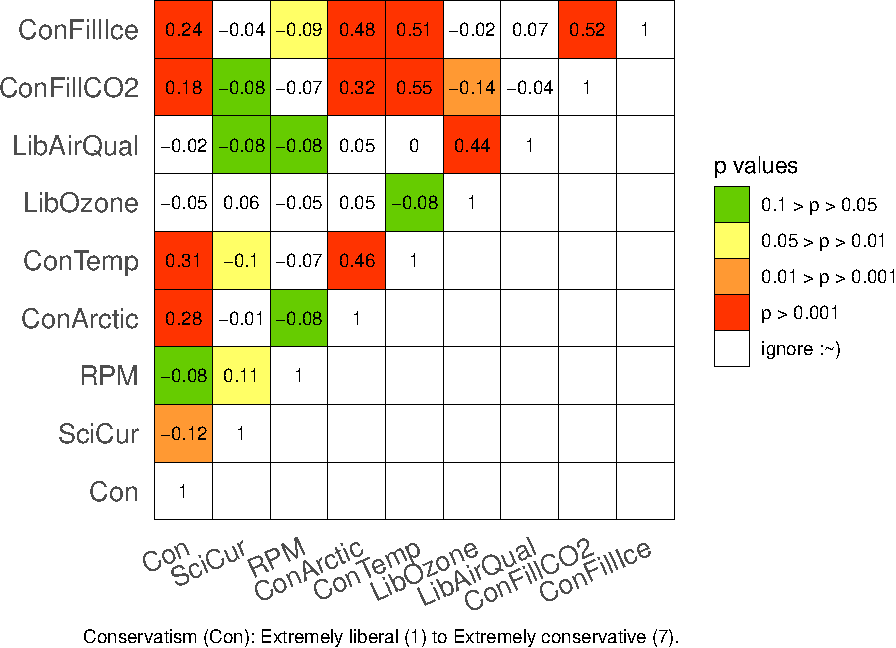
\includegraphics{DESC-TODAY_files/figure-latex/cor-mat1-1.pdf}

\hypertarget{science-curiosity-and-rpm}{%
\subsection{Science curiosity and RPM}\label{science-curiosity-and-rpm}}

\textbf{Grouped by ideology}

\begin{tabular}{>{}l||>{}c|c|>{}c|>{}c||>{}c|c|>{}c|c}
\hline
\multicolumn{1}{c|}{ } & \multicolumn{4}{c|}{Conservative} & \multicolumn{4}{c}{Liberal} \\
\cline{2-5} \cline{6-9}
  & Mean & SE & Min & Max & Mean & SE & Min & Max\\
\hline
\textbf{SciCuriosity} & \cellcolor{lightgray}{24.12} & 0.38 & \cellcolor{lightgray}{9} & 43 & \cellcolor{lightgray}{25.25} & 0.35 & \cellcolor{lightgray}{9} & 44\\
\hline
\textbf{RPM} & \cellcolor{lightgray}{5.55} & 0.10 & \cellcolor{lightgray}{1} & 10 & \cellcolor{lightgray}{5.71} & 0.10 & \cellcolor{lightgray}{1} & 10\\
\hline
\end{tabular}

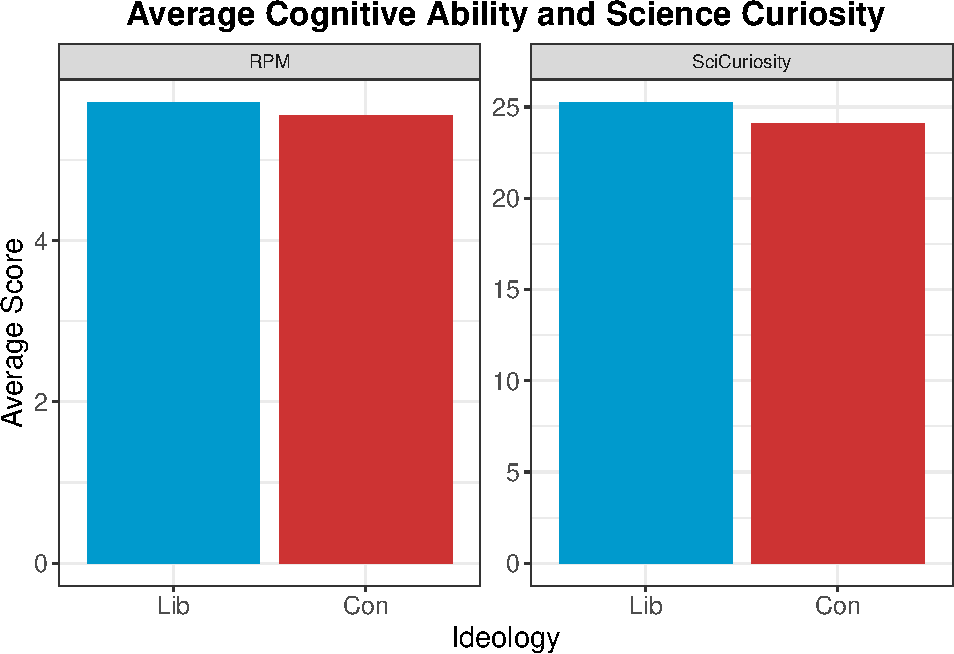
\includegraphics{DESC-TODAY_files/figure-latex/cont-plot-1.pdf}

\hypertarget{motivated-reasoning-items}{%
\subsection{Motivated reasoning items}\label{motivated-reasoning-items}}

\textbf{Grouped by ideology}

\begin{tabular}{>{}l||>{}c|c|>{}c|>{}c||>{}c|c|>{}c|c}
\hline
\multicolumn{1}{c|}{ } & \multicolumn{4}{c|}{Conservative} & \multicolumn{4}{c}{Liberal} \\
\cline{2-5} \cline{6-9}
  & Mean & SE & Min & Max & Mean & SE & Min & Max\\
\hline
\textbf{ConArctic} & \cellcolor{lightgray}{-1.07} & 0.09 & \cellcolor{lightgray}{-3} & 3 & \cellcolor{lightgray}{-1.73} & 0.07 & \cellcolor{lightgray}{-3} & 3\\
\hline
\textbf{ConTemp} & \cellcolor{lightgray}{-1.37} & 0.08 & \cellcolor{lightgray}{-3} & 3 & \cellcolor{lightgray}{-1.97} & 0.06 & \cellcolor{lightgray}{-3} & 2\\
\hline
\textbf{LibOzone} & \cellcolor{lightgray}{-0.32} & 0.09 & \cellcolor{lightgray}{-3} & 3 & \cellcolor{lightgray}{-0.21} & 0.09 & \cellcolor{lightgray}{-3} & 3\\
\hline
\textbf{LibAir} & \cellcolor{lightgray}{-0.85} & 0.10 & \cellcolor{lightgray}{-3} & 3 & \cellcolor{lightgray}{-0.81} & 0.10 & \cellcolor{lightgray}{-3} & 3\\
\hline
\textbf{ConFillIce} & \cellcolor{lightgray}{-1.83} & 0.09 & \cellcolor{lightgray}{-3} & 3 & \cellcolor{lightgray}{-2.33} & 0.06 & \cellcolor{lightgray}{-3} & 3\\
\hline
\textbf{FillBacteria} & \cellcolor{lightgray}{-0.16} & 0.08 & \cellcolor{lightgray}{-3} & 3 & \cellcolor{lightgray}{-0.35} & 0.08 & \cellcolor{lightgray}{-3} & 3\\
\hline
\textbf{FillQuake} & \cellcolor{lightgray}{0.29} & 0.03 & \cellcolor{lightgray}{0} & 1 & \cellcolor{lightgray}{0.33} & 0.03 & \cellcolor{lightgray}{0} & 1\\
\hline
\end{tabular}

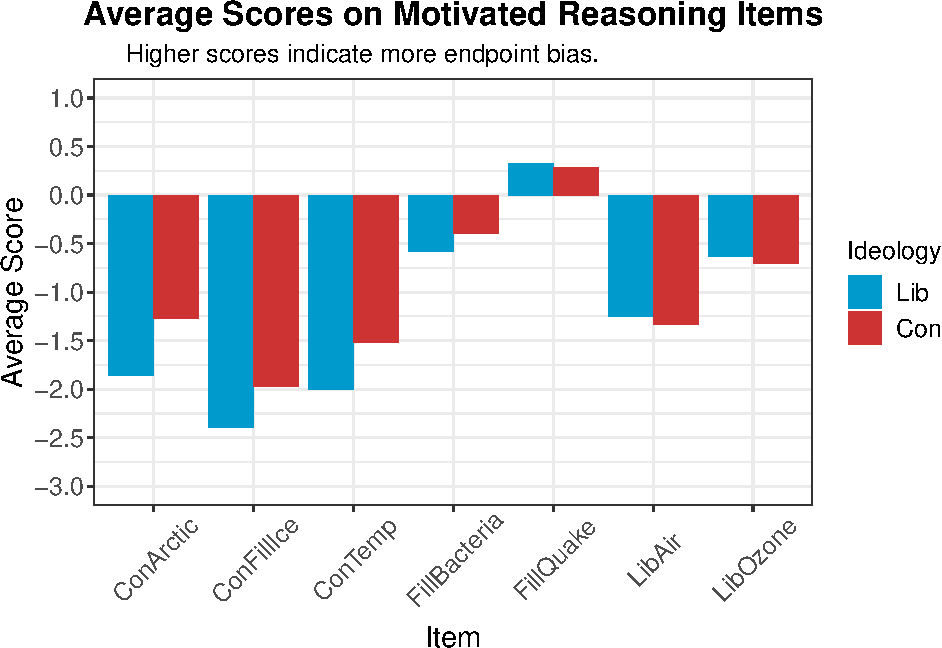
\includegraphics{DESC-TODAY_files/figure-latex/eb-ideo-plot-1.pdf}

\hypertarget{way-int.-means}{%
\section{``3-way int.'' means}\label{way-int.-means}}

\begin{tabular}{>{}c|c|>{}c||c|>{}c||c|>{}c||c|>{}c||c|c}
\hline
\multicolumn{3}{c|}{ } & \multicolumn{4}{c|}{Conservative} & \multicolumn{4}{c}{Liberal} \\
\cline{4-7} \cline{8-11}
 & SciCur & RPM & Con1\_M & Con1\_SE & Con2\_M & Con2\_SE & Lib1\_M & Lib1\_SE & Lib2\_M & Lib2\_SE\\
\hline
\cellcolor{maroon}{\textcolor{white}{\textbf{Con}}} & \cellcolor{lightgray}{High} & \cellcolor{lightgray}{High} & \cellcolor{lightgray}{-1.05} & \cellcolor{lightgray}{0.18} & \cellcolor{lightgray}{-1.38} & \cellcolor{lightgray}{0.17} & \cellcolor{lightgray}{-0.14} & \cellcolor{lightgray}{0.16} & \cellcolor{lightgray}{-0.92} & \cellcolor{lightgray}{0.19}\\
\hline
\cellcolor{maroon}{\textcolor{white}{\textbf{Con}}} & \cellcolor{lightgray}{High} & \cellcolor{lightgray}{Low} & \cellcolor{lightgray}{-1.00} & \cellcolor{lightgray}{0.22} & \cellcolor{lightgray}{-1.31} & \cellcolor{lightgray}{0.19} & \cellcolor{lightgray}{-0.33} & \cellcolor{lightgray}{0.24} & \cellcolor{lightgray}{-0.98} & \cellcolor{lightgray}{0.24}\\
\hline
\cellcolor{maroon}{\textcolor{white}{\textbf{Con}}} & Low & High & -1.05 & 0.15 & -1.23 & 0.14 & -0.52 & 0.14 & -0.80 & 0.18\\
\hline
\cellcolor{maroon}{\textcolor{white}{\textbf{Con}}} & Low & Low & -1.19 & 0.18 & -1.58 & 0.16 & -0.28 & 0.22 & -0.68 & 0.23\\
\hline
\cellcolor{royalblue}{\textcolor{white}{\textbf{Lib}}} & \cellcolor{lightgray}{High} & \cellcolor{lightgray}{High} & \cellcolor{lightgray}{-1.85} & \cellcolor{lightgray}{0.11} & \cellcolor{lightgray}{-2.14} & \cellcolor{lightgray}{0.09} & \cellcolor{lightgray}{-0.27} & \cellcolor{lightgray}{0.14} & \cellcolor{lightgray}{-0.92} & \cellcolor{lightgray}{0.17}\\
\hline
\cellcolor{royalblue}{\textcolor{white}{\textbf{Lib}}} & \cellcolor{lightgray}{High} & \cellcolor{lightgray}{Low} & \cellcolor{lightgray}{-1.45} & \cellcolor{lightgray}{0.20} & \cellcolor{lightgray}{-2.00} & \cellcolor{lightgray}{0.10} & \cellcolor{lightgray}{-0.02} & \cellcolor{lightgray}{0.20} & \cellcolor{lightgray}{-0.62} & \cellcolor{lightgray}{0.24}\\
\hline
\cellcolor{royalblue}{\textcolor{white}{\textbf{Lib}}} & Low & High & -1.88 & 0.12 & -2.15 & 0.10 & -0.08 & 0.21 & -0.75 & 0.20\\
\hline
\cellcolor{royalblue}{\textcolor{white}{\textbf{Lib}}} & Low & Low & -1.71 & 0.17 & -1.53 & 0.16 & -0.40 & 0.17 & -0.87 & 0.19\\
\hline
\multicolumn{11}{l}{\rule{0pt}{1em}\textit{Note: }}\\
\multicolumn{11}{l}{\rule{0pt}{1em}makecell[l]{* M = mean, SE = standard error \ * Item names: Con1 = arctic sea ice, Con2 = global temperature index, Lib1 = ozone layer hole, Lib2 = US air quality}}\\
\end{tabular}

\hypertarget{conservative-1-arctic}{%
\section{Conservative \#1: Arctic}\label{conservative-1-arctic}}

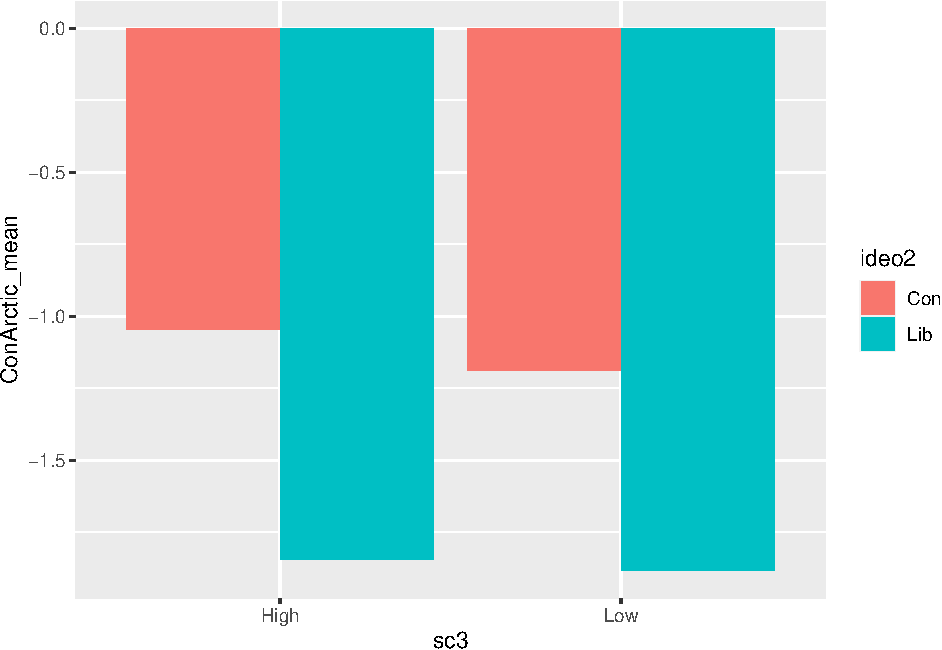
\includegraphics{DESC-TODAY_files/figure-latex/unnamed-chunk-1-1.pdf}

\begin{Shaded}
\begin{Highlighting}[]
\NormalTok{arcmod1 }\OtherTok{\textless{}{-}} \FunctionTok{lm}\NormalTok{(ConArctic }\SpecialCharTok{\textasciitilde{}} \DecValTok{1}\NormalTok{, }\AttributeTok{data =}\NormalTok{ dfd2\_lc)}
\FunctionTok{summary}\NormalTok{(arcmod1)}
\end{Highlighting}
\end{Shaded}

\begin{verbatim}
## 
## Call:
## lm(formula = ConArctic ~ 1, data = dfd2_lc)
## 
## Residuals:
##     Min      1Q  Median      3Q     Max 
## -1.5723 -0.5723 -0.5723  0.4277  4.4277 
## 
## Coefficients:
##             Estimate Std. Error t value Pr(>|t|)    
## (Intercept) -1.42770    0.05952  -23.99   <2e-16 ***
## ---
## Signif. codes:  0 '***' 0.001 '**' 0.01 '*' 0.05 '.' 0.1 ' ' 1
## 
## Residual standard error: 1.319 on 490 degrees of freedom
\end{verbatim}

\begin{Shaded}
\begin{Highlighting}[]
\NormalTok{arcmod2 }\OtherTok{\textless{}{-}} \FunctionTok{lm}\NormalTok{(ConArctic }\SpecialCharTok{\textasciitilde{}}\NormalTok{ rav\_scoredz, }\AttributeTok{data =}\NormalTok{ dfd2\_lc)}
\FunctionTok{summary}\NormalTok{(arcmod2)}
\end{Highlighting}
\end{Shaded}

\begin{verbatim}
## 
## Call:
## lm(formula = ConArctic ~ rav_scoredz, data = dfd2_lc)
## 
## Residuals:
##     Min      1Q  Median      3Q     Max 
## -1.8764 -0.6798 -0.4831  0.4513  4.3858 
## 
## Coefficients:
##             Estimate Std. Error t value Pr(>|t|)    
## (Intercept) -1.42549    0.05940 -23.997   <2e-16 ***
## rav_scoredz -0.10473    0.05993  -1.748   0.0811 .  
## ---
## Signif. codes:  0 '***' 0.001 '**' 0.01 '*' 0.05 '.' 0.1 ' ' 1
## 
## Residual standard error: 1.316 on 489 degrees of freedom
## Multiple R-squared:  0.006207,   Adjusted R-squared:  0.004175 
## F-statistic: 3.054 on 1 and 489 DF,  p-value: 0.08115
\end{verbatim}

\begin{Shaded}
\begin{Highlighting}[]
\FunctionTok{anova}\NormalTok{(arcmod1, arcmod2)}
\end{Highlighting}
\end{Shaded}

\begin{verbatim}
## Analysis of Variance Table
## 
## Model 1: ConArctic ~ 1
## Model 2: ConArctic ~ rav_scoredz
##   Res.Df    RSS Df Sum of Sq      F  Pr(>F)  
## 1    490 852.18                              
## 2    489 846.89  1    5.2899 3.0544 0.08115 .
## ---
## Signif. codes:  0 '***' 0.001 '**' 0.01 '*' 0.05 '.' 0.1 ' ' 1
\end{verbatim}

\begin{Shaded}
\begin{Highlighting}[]
\NormalTok{arcmod3 }\OtherTok{\textless{}{-}} \FunctionTok{lm}\NormalTok{(ConArctic }\SpecialCharTok{\textasciitilde{}}\NormalTok{ sc\_scoredz }\SpecialCharTok{+}\NormalTok{ rav\_scoredz, }\AttributeTok{data =}\NormalTok{ dfd2\_lc)}
\FunctionTok{summary}\NormalTok{(arcmod3)}
\end{Highlighting}
\end{Shaded}

\begin{verbatim}
## 
## Call:
## lm(formula = ConArctic ~ sc_scoredz + rav_scoredz, data = dfd2_lc)
## 
## Residuals:
##     Min      1Q  Median      3Q     Max 
## -1.8788 -0.6782 -0.4836  0.4514  4.3839 
## 
## Coefficients:
##              Estimate Std. Error t value Pr(>|t|)    
## (Intercept) -1.425486   0.059466 -23.972   <2e-16 ***
## sc_scoredz  -0.002092   0.061643  -0.034   0.9729    
## rav_scoredz -0.104508   0.060348  -1.732   0.0839 .  
## ---
## Signif. codes:  0 '***' 0.001 '**' 0.01 '*' 0.05 '.' 0.1 ' ' 1
## 
## Residual standard error: 1.317 on 488 degrees of freedom
## Multiple R-squared:  0.00621,    Adjusted R-squared:  0.002137 
## F-statistic: 1.525 on 2 and 488 DF,  p-value: 0.2187
\end{verbatim}

\begin{Shaded}
\begin{Highlighting}[]
\FunctionTok{anova}\NormalTok{(arcmod1, arcmod3)}
\end{Highlighting}
\end{Shaded}

\begin{verbatim}
## Analysis of Variance Table
## 
## Model 1: ConArctic ~ 1
## Model 2: ConArctic ~ sc_scoredz + rav_scoredz
##   Res.Df    RSS Df Sum of Sq      F Pr(>F)
## 1    490 852.18                           
## 2    488 846.89  2    5.2919 1.5247 0.2187
\end{verbatim}

\begin{Shaded}
\begin{Highlighting}[]
\NormalTok{arcmod4 }\OtherTok{\textless{}{-}} \FunctionTok{lm}\NormalTok{(ConArctic }\SpecialCharTok{\textasciitilde{}}\NormalTok{ ArcticCong }\SpecialCharTok{+}\NormalTok{ sc\_scoredz }\SpecialCharTok{+}\NormalTok{ rav\_scoredz, }\AttributeTok{data =}\NormalTok{ dfd2\_lc)}
\FunctionTok{summary}\NormalTok{(arcmod4)}
\end{Highlighting}
\end{Shaded}

\begin{verbatim}
## 
## Call:
## lm(formula = ConArctic ~ ArcticCong + sc_scoredz + rav_scoredz, 
##     data = dfd2_lc)
## 
## Residuals:
##     Min      1Q  Median      3Q     Max 
## -2.1985 -0.9416 -0.2329  0.6405  4.5164 
## 
## Coefficients:
##             Estimate Std. Error t value Pr(>|t|)    
## (Intercept) -1.72874    0.07874 -21.954  < 2e-16 ***
## ArcticCong   0.65778    0.11632   5.655 2.66e-08 ***
## sc_scoredz   0.02956    0.06004   0.492    0.623    
## rav_scoredz -0.09122    0.05857  -1.558    0.120    
## ---
## Signif. codes:  0 '***' 0.001 '**' 0.01 '*' 0.05 '.' 0.1 ' ' 1
## 
## Residual standard error: 1.277 on 487 degrees of freedom
## Multiple R-squared:  0.06745,    Adjusted R-squared:  0.0617 
## F-statistic: 11.74 on 3 and 487 DF,  p-value: 1.942e-07
\end{verbatim}

\begin{Shaded}
\begin{Highlighting}[]
\FunctionTok{anova}\NormalTok{(arcmod1, arcmod4)}
\end{Highlighting}
\end{Shaded}

\begin{verbatim}
## Analysis of Variance Table
## 
## Model 1: ConArctic ~ 1
## Model 2: ConArctic ~ ArcticCong + sc_scoredz + rav_scoredz
##   Res.Df    RSS Df Sum of Sq      F    Pr(>F)    
## 1    490 852.18                                  
## 2    487 794.71  3    57.476 11.741 1.942e-07 ***
## ---
## Signif. codes:  0 '***' 0.001 '**' 0.01 '*' 0.05 '.' 0.1 ' ' 1
\end{verbatim}

\hypertarget{conservative-2-temp}{%
\section{Conservative \#2: Temp}\label{conservative-2-temp}}

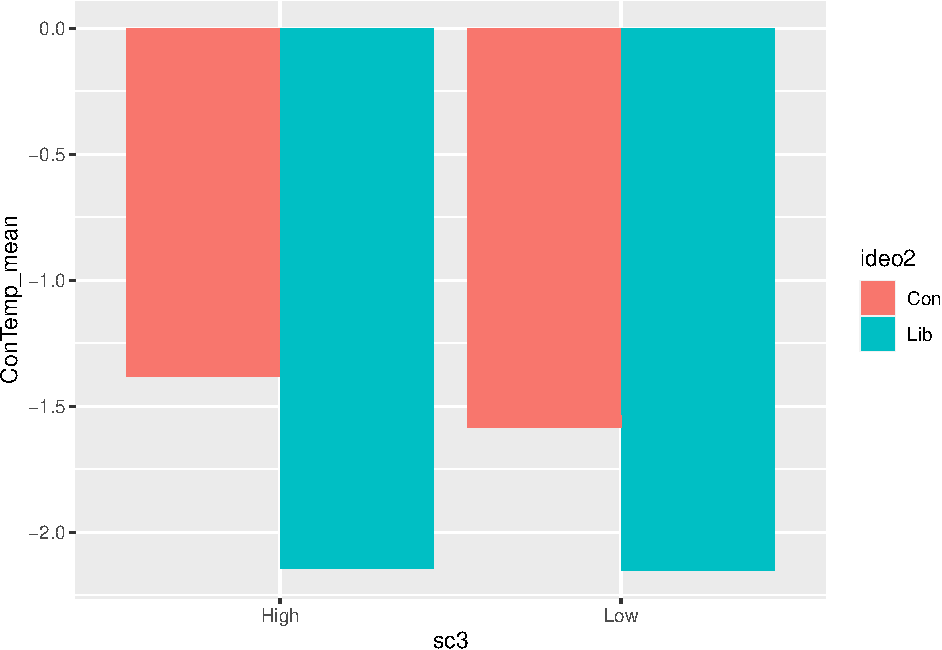
\includegraphics{DESC-TODAY_files/figure-latex/unnamed-chunk-3-1.pdf}

\begin{Shaded}
\begin{Highlighting}[]
\NormalTok{tempmod1 }\OtherTok{\textless{}{-}} \FunctionTok{lm}\NormalTok{(ConTemp }\SpecialCharTok{\textasciitilde{}} \DecValTok{1}\NormalTok{, }\AttributeTok{data =}\NormalTok{ dfd2\_lc)}
\FunctionTok{summary}\NormalTok{(tempmod1)}
\end{Highlighting}
\end{Shaded}

\begin{verbatim}
## 
## Call:
## lm(formula = ConTemp ~ 1, data = dfd2_lc)
## 
## Residuals:
##     Min      1Q  Median      3Q     Max 
## -1.3055 -0.3055 -0.3055  0.6945  4.6945 
## 
## Coefficients:
##             Estimate Std. Error t value Pr(>|t|)    
## (Intercept) -1.69450    0.05126  -33.06   <2e-16 ***
## ---
## Signif. codes:  0 '***' 0.001 '**' 0.01 '*' 0.05 '.' 0.1 ' ' 1
## 
## Residual standard error: 1.136 on 490 degrees of freedom
\end{verbatim}

\begin{Shaded}
\begin{Highlighting}[]
\NormalTok{tempmod2 }\OtherTok{\textless{}{-}} \FunctionTok{lm}\NormalTok{(ConTemp }\SpecialCharTok{\textasciitilde{}}\NormalTok{ rav\_scoredz, }\AttributeTok{data =}\NormalTok{ dfd2\_lc)}
\FunctionTok{summary}\NormalTok{(tempmod2)}
\end{Highlighting}
\end{Shaded}

\begin{verbatim}
## 
## Call:
## lm(formula = ConTemp ~ rav_scoredz, data = dfd2_lc)
## 
## Residuals:
##     Min      1Q  Median      3Q     Max 
## -1.5464 -0.4425 -0.2868  0.6613  4.6094 
## 
## Coefficients:
##             Estimate Std. Error t value Pr(>|t|)    
## (Intercept) -1.69276    0.05119 -33.069   <2e-16 ***
## rav_scoredz -0.08296    0.05164  -1.607    0.109    
## ---
## Signif. codes:  0 '***' 0.001 '**' 0.01 '*' 0.05 '.' 0.1 ' ' 1
## 
## Residual standard error: 1.134 on 489 degrees of freedom
## Multiple R-squared:  0.00525,    Adjusted R-squared:  0.003216 
## F-statistic: 2.581 on 1 and 489 DF,  p-value: 0.1088
\end{verbatim}

\begin{Shaded}
\begin{Highlighting}[]
\FunctionTok{anova}\NormalTok{(tempmod1, tempmod2)}
\end{Highlighting}
\end{Shaded}

\begin{verbatim}
## Analysis of Variance Table
## 
## Model 1: ConTemp ~ 1
## Model 2: ConTemp ~ rav_scoredz
##   Res.Df    RSS Df Sum of Sq     F Pr(>F)
## 1    490 632.18                          
## 2    489 628.86  1    3.3192 2.581 0.1088
\end{verbatim}

\begin{Shaded}
\begin{Highlighting}[]
\NormalTok{tempmod3 }\OtherTok{\textless{}{-}} \FunctionTok{lm}\NormalTok{(ConTemp }\SpecialCharTok{\textasciitilde{}}\NormalTok{ sc\_scoredz }\SpecialCharTok{+}\NormalTok{ rav\_scoredz, }\AttributeTok{data =}\NormalTok{ dfd2\_lc)}
\FunctionTok{summary}\NormalTok{(tempmod3)}
\end{Highlighting}
\end{Shaded}

\begin{verbatim}
## 
## Call:
## lm(formula = ConTemp ~ sc_scoredz + rav_scoredz, data = dfd2_lc)
## 
## Residuals:
##     Min      1Q  Median      3Q     Max 
## -1.6735 -0.4882 -0.2660  0.6194  4.6819 
## 
## Coefficients:
##             Estimate Std. Error t value Pr(>|t|)    
## (Intercept) -1.69229    0.05102 -33.172   <2e-16 ***
## sc_scoredz  -0.11015    0.05288  -2.083   0.0378 *  
## rav_scoredz -0.07119    0.05177  -1.375   0.1698    
## ---
## Signif. codes:  0 '***' 0.001 '**' 0.01 '*' 0.05 '.' 0.1 ' ' 1
## 
## Residual standard error: 1.13 on 488 degrees of freedom
## Multiple R-squared:  0.01402,    Adjusted R-squared:  0.009974 
## F-statistic: 3.468 on 2 and 488 DF,  p-value: 0.03194
\end{verbatim}

\begin{Shaded}
\begin{Highlighting}[]
\FunctionTok{anova}\NormalTok{(tempmod1, tempmod3)}
\end{Highlighting}
\end{Shaded}

\begin{verbatim}
## Analysis of Variance Table
## 
## Model 1: ConTemp ~ 1
## Model 2: ConTemp ~ sc_scoredz + rav_scoredz
##   Res.Df    RSS Df Sum of Sq      F  Pr(>F)  
## 1    490 632.18                              
## 2    488 623.32  2    8.8601 3.4683 0.03194 *
## ---
## Signif. codes:  0 '***' 0.001 '**' 0.01 '*' 0.05 '.' 0.1 ' ' 1
\end{verbatim}

\begin{Shaded}
\begin{Highlighting}[]
\NormalTok{tempmod4 }\OtherTok{\textless{}{-}} \FunctionTok{lm}\NormalTok{(ConTemp }\SpecialCharTok{\textasciitilde{}}\NormalTok{ TempCong }\SpecialCharTok{+}\NormalTok{ sc\_scoredz }\SpecialCharTok{+}\NormalTok{ rav\_scoredz, }\AttributeTok{data =}\NormalTok{ dfd2\_lc)}
\FunctionTok{summary}\NormalTok{(tempmod4)}
\end{Highlighting}
\end{Shaded}

\begin{verbatim}
## 
## Call:
## lm(formula = ConTemp ~ TempCong + sc_scoredz + rav_scoredz, data = dfd2_lc)
## 
## Residuals:
##     Min      1Q  Median      3Q     Max 
## -1.9102 -0.7079 -0.0741  0.4027  4.3675 
## 
## Coefficients:
##             Estimate Std. Error t value Pr(>|t|)    
## (Intercept) -1.95804    0.06746 -29.025  < 2e-16 ***
## TempCong     0.57643    0.09965   5.785  1.3e-08 ***
## sc_scoredz  -0.08241    0.05143  -1.602    0.110    
## rav_scoredz -0.05954    0.05017  -1.187    0.236    
## ---
## Signif. codes:  0 '***' 0.001 '**' 0.01 '*' 0.05 '.' 0.1 ' ' 1
## 
## Residual standard error: 1.094 on 487 degrees of freedom
## Multiple R-squared:  0.07741,    Adjusted R-squared:  0.07172 
## F-statistic: 13.62 on 3 and 487 DF,  p-value: 1.517e-08
\end{verbatim}

\begin{Shaded}
\begin{Highlighting}[]
\FunctionTok{anova}\NormalTok{(tempmod3, tempmod4)}
\end{Highlighting}
\end{Shaded}

\begin{verbatim}
## Analysis of Variance Table
## 
## Model 1: ConTemp ~ sc_scoredz + rav_scoredz
## Model 2: ConTemp ~ TempCong + sc_scoredz + rav_scoredz
##   Res.Df    RSS Df Sum of Sq      F    Pr(>F)    
## 1    488 623.32                                  
## 2    487 583.24  1    40.075 33.462 1.301e-08 ***
## ---
## Signif. codes:  0 '***' 0.001 '**' 0.01 '*' 0.05 '.' 0.1 ' ' 1
\end{verbatim}

\hypertarget{liberal-1-ozone}{%
\section{Liberal \#1: Ozone}\label{liberal-1-ozone}}

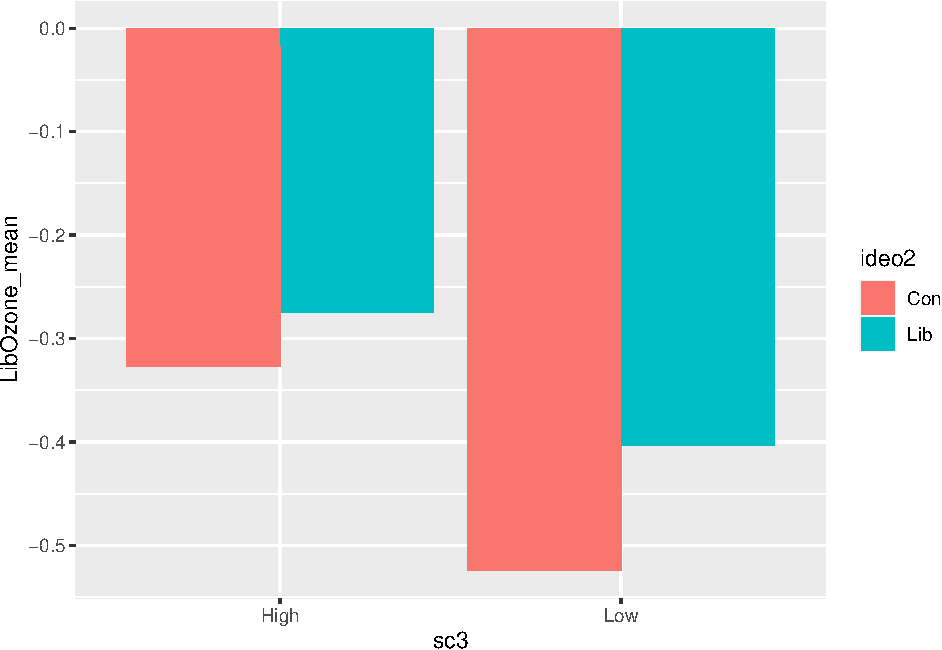
\includegraphics{DESC-TODAY_files/figure-latex/unnamed-chunk-5-1.pdf}

\begin{Shaded}
\begin{Highlighting}[]
\NormalTok{ozmod1 }\OtherTok{\textless{}{-}} \FunctionTok{lm}\NormalTok{(LibOzone }\SpecialCharTok{\textasciitilde{}} \DecValTok{1}\NormalTok{, }\AttributeTok{data =}\NormalTok{ dfd2\_lc)}
\FunctionTok{summary}\NormalTok{(ozmod1)}
\end{Highlighting}
\end{Shaded}

\begin{verbatim}
## 
## Call:
## lm(formula = LibOzone ~ 1, data = dfd2_lc)
## 
## Residuals:
##     Min      1Q  Median      3Q     Max 
## -2.7413 -0.7413 -0.7413  1.2587  3.2587 
## 
## Coefficients:
##             Estimate Std. Error t value Pr(>|t|)    
## (Intercept) -0.25866    0.06383  -4.052 5.89e-05 ***
## ---
## Signif. codes:  0 '***' 0.001 '**' 0.01 '*' 0.05 '.' 0.1 ' ' 1
## 
## Residual standard error: 1.414 on 490 degrees of freedom
\end{verbatim}

\begin{Shaded}
\begin{Highlighting}[]
\NormalTok{ozmod2 }\OtherTok{\textless{}{-}} \FunctionTok{lm}\NormalTok{(LibOzone }\SpecialCharTok{\textasciitilde{}}\NormalTok{ rav\_scoredz, }\AttributeTok{data =}\NormalTok{ dfd2\_lc)}
\FunctionTok{summary}\NormalTok{(ozmod2)}
\end{Highlighting}
\end{Shaded}

\begin{verbatim}
## 
## Call:
## lm(formula = LibOzone ~ rav_scoredz, data = dfd2_lc)
## 
## Residuals:
##     Min      1Q  Median      3Q     Max 
## -2.8974 -0.7688 -0.6401  1.2312  3.3599 
## 
## Coefficients:
##             Estimate Std. Error t value Pr(>|t|)    
## (Intercept) -0.25721    0.06383  -4.029 6.48e-05 ***
## rav_scoredz -0.06850    0.06439  -1.064    0.288    
## ---
## Signif. codes:  0 '***' 0.001 '**' 0.01 '*' 0.05 '.' 0.1 ' ' 1
## 
## Residual standard error: 1.414 on 489 degrees of freedom
## Multiple R-squared:  0.002309,   Adjusted R-squared:  0.0002684 
## F-statistic: 1.132 on 1 and 489 DF,  p-value: 0.288
\end{verbatim}

\begin{Shaded}
\begin{Highlighting}[]
\FunctionTok{anova}\NormalTok{(ozmod1, ozmod2)}
\end{Highlighting}
\end{Shaded}

\begin{verbatim}
## Analysis of Variance Table
## 
## Model 1: LibOzone ~ 1
## Model 2: LibOzone ~ rav_scoredz
##   Res.Df    RSS Df Sum of Sq      F Pr(>F)
## 1    490 980.15                           
## 2    489 977.89  1    2.2628 1.1315  0.288
\end{verbatim}

\begin{Shaded}
\begin{Highlighting}[]
\NormalTok{ozmod3 }\OtherTok{\textless{}{-}} \FunctionTok{lm}\NormalTok{(LibOzone }\SpecialCharTok{\textasciitilde{}}\NormalTok{ sc\_scoredz }\SpecialCharTok{+}\NormalTok{ rav\_scoredz, }\AttributeTok{data =}\NormalTok{ dfd2\_lc)}
\FunctionTok{summary}\NormalTok{(ozmod3)}
\end{Highlighting}
\end{Shaded}

\begin{verbatim}
## 
## Call:
## lm(formula = LibOzone ~ sc_scoredz + rav_scoredz, data = dfd2_lc)
## 
## Residuals:
##     Min      1Q  Median      3Q     Max 
## -2.9220 -0.8104 -0.6018  1.2041  3.4952 
## 
## Coefficients:
##             Estimate Std. Error t value Pr(>|t|)    
## (Intercept) -0.25761    0.06376  -4.040 6.21e-05 ***
## sc_scoredz   0.09501    0.06610   1.437    0.151    
## rav_scoredz -0.07865    0.06471  -1.215    0.225    
## ---
## Signif. codes:  0 '***' 0.001 '**' 0.01 '*' 0.05 '.' 0.1 ' ' 1
## 
## Residual standard error: 1.413 on 488 degrees of freedom
## Multiple R-squared:  0.006514,   Adjusted R-squared:  0.002443 
## F-statistic:   1.6 on 2 and 488 DF,  p-value: 0.203
\end{verbatim}

\begin{Shaded}
\begin{Highlighting}[]
\FunctionTok{anova}\NormalTok{(ozmod1, ozmod3)}
\end{Highlighting}
\end{Shaded}

\begin{verbatim}
## Analysis of Variance Table
## 
## Model 1: LibOzone ~ 1
## Model 2: LibOzone ~ sc_scoredz + rav_scoredz
##   Res.Df    RSS Df Sum of Sq      F Pr(>F)
## 1    490 980.15                           
## 2    488 973.77  2     6.385 1.5999  0.203
\end{verbatim}

\begin{Shaded}
\begin{Highlighting}[]
\NormalTok{ozmod4 }\OtherTok{\textless{}{-}} \FunctionTok{lm}\NormalTok{(LibOzone }\SpecialCharTok{\textasciitilde{}}\NormalTok{ OzoneCong }\SpecialCharTok{+}\NormalTok{ sc\_scoredz }\SpecialCharTok{+}\NormalTok{ rav\_scoredz, }\AttributeTok{data =}\NormalTok{ dfd2\_lc)}
\FunctionTok{summary}\NormalTok{(ozmod4)}
\end{Highlighting}
\end{Shaded}

\begin{verbatim}
## 
## Call:
## lm(formula = LibOzone ~ OzoneCong + sc_scoredz + rav_scoredz, 
##     data = dfd2_lc)
## 
## Residuals:
##     Min      1Q  Median      3Q     Max 
## -2.8704 -0.8270 -0.5915  1.1704  3.4375 
## 
## Coefficients:
##             Estimate Std. Error t value Pr(>|t|)    
## (Intercept) -0.31255    0.09423  -3.317 0.000978 ***
## OzoneCong    0.10193    0.12868   0.792 0.428669    
## sc_scoredz   0.09010    0.06641   1.357 0.175519    
## rav_scoredz -0.08071    0.06479  -1.246 0.213432    
## ---
## Signif. codes:  0 '***' 0.001 '**' 0.01 '*' 0.05 '.' 0.1 ' ' 1
## 
## Residual standard error: 1.413 on 487 degrees of freedom
## Multiple R-squared:  0.007793,   Adjusted R-squared:  0.001681 
## F-statistic: 1.275 on 3 and 487 DF,  p-value: 0.2823
\end{verbatim}

\begin{Shaded}
\begin{Highlighting}[]
\FunctionTok{anova}\NormalTok{(ozmod1, ozmod4)}
\end{Highlighting}
\end{Shaded}

\begin{verbatim}
## Analysis of Variance Table
## 
## Model 1: LibOzone ~ 1
## Model 2: LibOzone ~ OzoneCong + sc_scoredz + rav_scoredz
##   Res.Df    RSS Df Sum of Sq     F Pr(>F)
## 1    490 980.15                          
## 2    487 972.51  3    7.6381 1.275 0.2823
\end{verbatim}

\hypertarget{liberal-2-air-quality}{%
\section{Liberal \#2: Air Quality}\label{liberal-2-air-quality}}

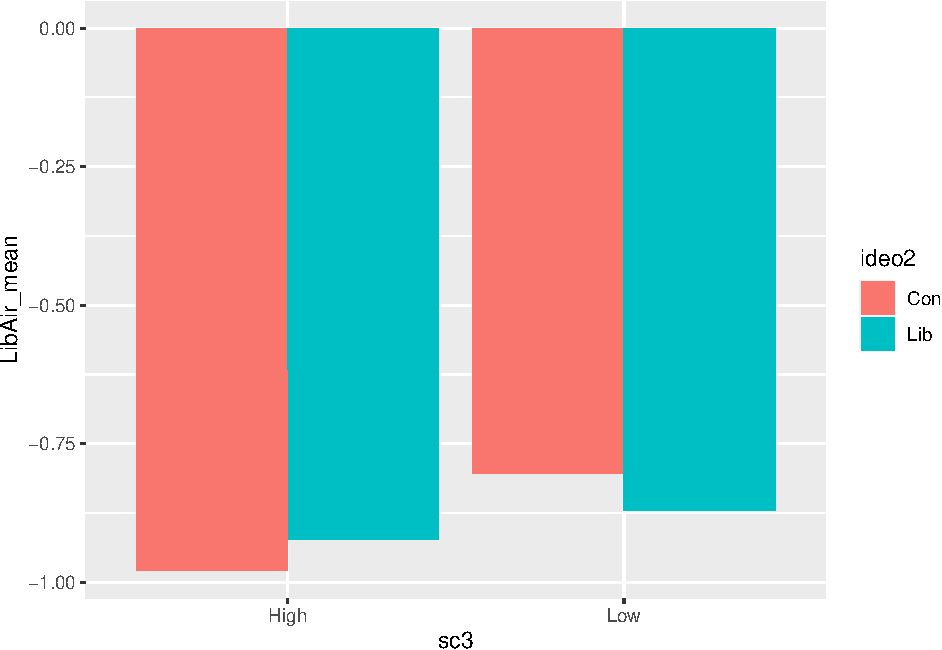
\includegraphics{DESC-TODAY_files/figure-latex/unnamed-chunk-7-1.pdf}

\begin{Shaded}
\begin{Highlighting}[]
\NormalTok{airmod1 }\OtherTok{\textless{}{-}} \FunctionTok{lm}\NormalTok{(LibAir }\SpecialCharTok{\textasciitilde{}} \DecValTok{1}\NormalTok{, }\AttributeTok{data =}\NormalTok{ dfd2\_lc)}
\FunctionTok{summary}\NormalTok{(airmod1)}
\end{Highlighting}
\end{Shaded}

\begin{verbatim}
## 
## Call:
## lm(formula = LibAir ~ 1, data = dfd2_lc)
## 
## Residuals:
##     Min      1Q  Median      3Q     Max 
## -2.1752 -1.1752 -0.1752  0.8248  3.8248 
## 
## Coefficients:
##             Estimate Std. Error t value Pr(>|t|)    
## (Intercept) -0.82485    0.07176  -11.49   <2e-16 ***
## ---
## Signif. codes:  0 '***' 0.001 '**' 0.01 '*' 0.05 '.' 0.1 ' ' 1
## 
## Residual standard error: 1.59 on 490 degrees of freedom
\end{verbatim}

\begin{Shaded}
\begin{Highlighting}[]
\NormalTok{airmod2 }\OtherTok{\textless{}{-}} \FunctionTok{lm}\NormalTok{(LibAir }\SpecialCharTok{\textasciitilde{}}\NormalTok{ rav\_scoredz, }\AttributeTok{data =}\NormalTok{ dfd2\_lc)}
\FunctionTok{summary}\NormalTok{(airmod2)}
\end{Highlighting}
\end{Shaded}

\begin{verbatim}
## 
## Call:
## lm(formula = LibAir ~ rav_scoredz, data = dfd2_lc)
## 
## Residuals:
##     Min      1Q  Median      3Q     Max 
## -2.5557 -1.1456 -0.3096  0.9365  4.0185 
## 
## Coefficients:
##             Estimate Std. Error t value Pr(>|t|)    
## (Intercept) -0.82209    0.07161 -11.480   <2e-16 ***
## rav_scoredz -0.13107    0.07224  -1.814   0.0702 .  
## ---
## Signif. codes:  0 '***' 0.001 '**' 0.01 '*' 0.05 '.' 0.1 ' ' 1
## 
## Residual standard error: 1.586 on 489 degrees of freedom
## Multiple R-squared:  0.006687,   Adjusted R-squared:  0.004656 
## F-statistic: 3.292 on 1 and 489 DF,  p-value: 0.07023
\end{verbatim}

\begin{Shaded}
\begin{Highlighting}[]
\FunctionTok{anova}\NormalTok{(airmod1, airmod2)}
\end{Highlighting}
\end{Shaded}

\begin{verbatim}
## Analysis of Variance Table
## 
## Model 1: LibAir ~ 1
## Model 2: LibAir ~ rav_scoredz
##   Res.Df    RSS Df Sum of Sq      F  Pr(>F)  
## 1    490 1238.9                              
## 2    489 1230.7  1    8.2851 3.2921 0.07023 .
## ---
## Signif. codes:  0 '***' 0.001 '**' 0.01 '*' 0.05 '.' 0.1 ' ' 1
\end{verbatim}

\begin{Shaded}
\begin{Highlighting}[]
\NormalTok{airmod3 }\OtherTok{\textless{}{-}} \FunctionTok{lm}\NormalTok{(LibAir }\SpecialCharTok{\textasciitilde{}}\NormalTok{ sc\_scoredz }\SpecialCharTok{+}\NormalTok{ rav\_scoredz, }\AttributeTok{data =}\NormalTok{ dfd2\_lc)}
\FunctionTok{summary}\NormalTok{(airmod3)}
\end{Highlighting}
\end{Shaded}

\begin{verbatim}
## 
## Call:
## lm(formula = LibAir ~ sc_scoredz + rav_scoredz, data = dfd2_lc)
## 
## Residuals:
##     Min      1Q  Median      3Q     Max 
## -2.6877 -1.1600 -0.3303  1.0284  4.1016 
## 
## Coefficients:
##             Estimate Std. Error t value Pr(>|t|)    
## (Intercept) -0.82161    0.07151 -11.490   <2e-16 ***
## sc_scoredz  -0.11439    0.07413  -1.543    0.123    
## rav_scoredz -0.11884    0.07257  -1.638    0.102    
## ---
## Signif. codes:  0 '***' 0.001 '**' 0.01 '*' 0.05 '.' 0.1 ' ' 1
## 
## Residual standard error: 1.584 on 488 degrees of freedom
## Multiple R-squared:  0.01151,    Adjusted R-squared:  0.00746 
## F-statistic: 2.841 on 2 and 488 DF,  p-value: 0.05931
\end{verbatim}

\begin{Shaded}
\begin{Highlighting}[]
\FunctionTok{anova}\NormalTok{(airmod1, airmod3)}
\end{Highlighting}
\end{Shaded}

\begin{verbatim}
## Analysis of Variance Table
## 
## Model 1: LibAir ~ 1
## Model 2: LibAir ~ sc_scoredz + rav_scoredz
##   Res.Df    RSS Df Sum of Sq      F  Pr(>F)  
## 1    490 1238.9                              
## 2    488 1224.7  2    14.261 2.8413 0.05931 .
## ---
## Signif. codes:  0 '***' 0.001 '**' 0.01 '*' 0.05 '.' 0.1 ' ' 1
\end{verbatim}

\begin{Shaded}
\begin{Highlighting}[]
\NormalTok{airmod4 }\OtherTok{\textless{}{-}} \FunctionTok{lm}\NormalTok{(LibAir }\SpecialCharTok{\textasciitilde{}}\NormalTok{ AirCong }\SpecialCharTok{+}\NormalTok{ sc\_scoredz }\SpecialCharTok{+}\NormalTok{ rav\_scoredz, }\AttributeTok{data =}\NormalTok{ dfd2\_lc)}
\FunctionTok{summary}\NormalTok{(airmod4)}
\end{Highlighting}
\end{Shaded}

\begin{verbatim}
## 
## Call:
## lm(formula = LibAir ~ AirCong + sc_scoredz + rav_scoredz, data = dfd2_lc)
## 
## Residuals:
##     Min      1Q  Median      3Q     Max 
## -2.6581 -1.1592 -0.3372  1.0363  4.0736 
## 
## Coefficients:
##             Estimate Std. Error t value Pr(>|t|)    
## (Intercept) -0.86049    0.10571  -8.140 3.34e-15 ***
## AirCong      0.07214    0.14436   0.500   0.6175    
## sc_scoredz  -0.11786    0.07451  -1.582   0.1143    
## rav_scoredz -0.12030    0.07268  -1.655   0.0986 .  
## ---
## Signif. codes:  0 '***' 0.001 '**' 0.01 '*' 0.05 '.' 0.1 ' ' 1
## 
## Residual standard error: 1.585 on 487 degrees of freedom
## Multiple R-squared:  0.01202,    Adjusted R-squared:  0.005931 
## F-statistic: 1.975 on 3 and 487 DF,  p-value: 0.1169
\end{verbatim}

\begin{Shaded}
\begin{Highlighting}[]
\FunctionTok{anova}\NormalTok{(airmod1, airmod4)}
\end{Highlighting}
\end{Shaded}

\begin{verbatim}
## Analysis of Variance Table
## 
## Model 1: LibAir ~ 1
## Model 2: LibAir ~ AirCong + sc_scoredz + rav_scoredz
##   Res.Df    RSS Df Sum of Sq      F Pr(>F)
## 1    490 1238.9                           
## 2    487 1224.0  3    14.889 1.9745 0.1169
\end{verbatim}

\end{document}
